\section{Design Concepts}\label{sec:appdesign}

We illustrate in the following language-independent design concepts,
providing a foundation to apply the COP model to different concrete
languages, as we further illustrate next. Throguhout this section and
the next, we refer to the wildelife tracking application described
earlier as a running example.

We define two key concepts:~\emph{i)} individual contexts, and
\emph{ii)} context groups. Contexts represent the different
environmental situations the system may encounter, and correspond to
behavioral variations associated to a given situation. As the
environment surrounding the system mutates, the software adapts
accordingly by activating given contexts. Context groups represent
collections of contexts sharing common characteristics; for example,
whenever the same functionality must adapt to changes in the
surrounding environment or the required adaptive behavior is
determined by the same environmental quantity. We argue that these
concepts are sufficient to capture a wide range of adaptive behaviors
in WSNs, and yet are largely independent of a specific programming
language.

% Programming in \conesc is intimately tied with environment-dependent behavior of
% the application and exploits two main concepts: \emph{i)} individual contexts
% and their transitions and \emph{ii)} context groups. The former represent
% different environment situations where a system may find itself. Each context
% maps to a separate state of the device or environment a system operates in. As
% the environment conditions change, a programmer initiates a context transition
% by \emph{activating} the corresponding context. A context group is a set of
% contexts sharing common characteristics and variations of the same
% functionality. Thus, whenever a transition between involved contexts occurs, it
% is determined by changes in one or more physical quantities.

\putfigure{caption=Wildlife tracking diagram.,label=fig:wtd}{
 \centering
 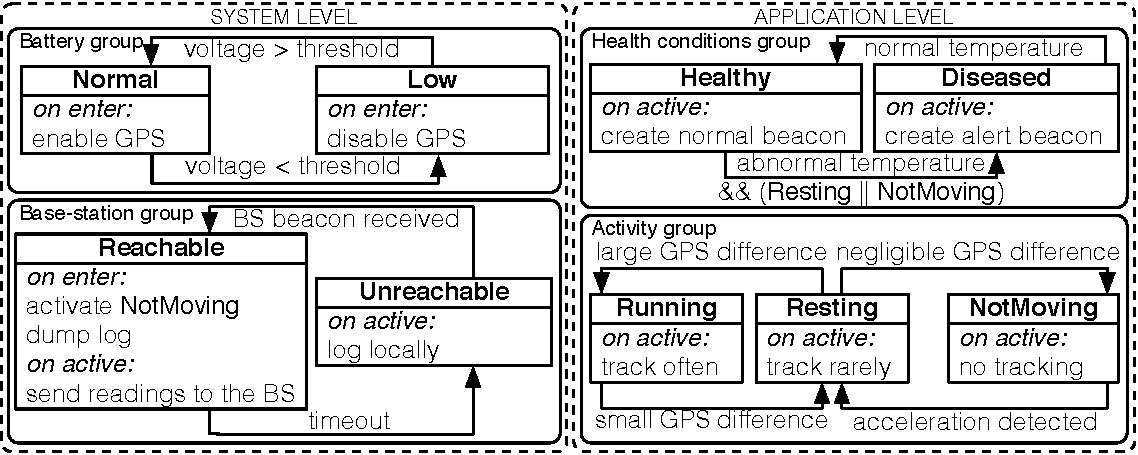
\includegraphics[width=\columnwidth]{pdf/wildlifetracking}
}

Fig.~\ref{fig:wtd} exemplifies how programmers use these concepts in
the design of the wildlife tracking application. Context groups are
defined to describe behavioral variations corresponding to different
battery levels and whether a node is within the communication range of
a base-station, as well as an animal's health conditions and
activity. Context groups are tagged as system-level or
application-level to discern application-specific functionality from
likely re-usable system services.

The contexts within a group define the individual behavioral
variations depending on the situation. For example, the function to
report sensor readings and contact traces must behave differently
depending on whether the base-station is reachable.  If so, the data
may be relayed immediately to the base-station using the radio. To
this end, the programmer activates context \emph{Reachable} within the
\emph{Base-station} group. Otherwise, the programmer activates context
\emph{Unreachable}, as the software must log the data locally; for
example, on flash. 

The contexts in a group are tied with transitions that
express the conditions triggering the context change. For example,
within the \emph{Base-station} group, the system transitions from
context \emph{Reachable} to \emph{Unreachable} whenever no beacons are
received from the base-station within a timeout. This entails
a node is out of the base-station communication range and the software
must adapt accordingly, that is, by locally storing the contact logs
instead of sending them over the radio.

% Orthogonal to application-level functionality, the system should transmit data
% to the Base Station (BS) or save readings locally depending on the BS
% availability. Whenever the latter is \emph{Unreachable}, a node logs data in
% internal memory, but should it receive a BS-beacon, the data is dumped to the
% BS. Crucially, the node runs on a battery, so the system should be aware of a
% battery status and disable GPS-module, which is power consuming, if the battery
% level is \emph{Low}.

The behavioral variations must not necessarily implement a complete
functionality on their own, but they may also serve other
functionality; for example, by providing context-dependent data. The
group \emph{Health conditions} is one such example. By using a body
temperature sensor, the system detects whether the animal is
\emph{Diseased} or \emph{Healthy}. The corresponding behavioral
variations implement two ways to build the radio beacon used as a
proximity sensor for detecting contacts between animals. If the animal
is \emph{Diseased}, additional information is added to the beacon for
understanding how the disease spreads. Either type of beacon is then
handed over to the radio stack for transmission.

The concepts we outlined suffice to organize the environment-dependent
functionality in a large class of WSN applications, as we further
argue in Section~\ref{sec:eval}. On the other hand, unlike the vast
majority of WSN programming approaches~\cite{mottola10:survey}, these
concepts remain largely decoupled from a concrete language
implementation. Although the following section describes a nesC-based
implementation---mainly motivated by the availability of a mature
toolchain---our design can be straightforwardly embedded within other
WSN languages. For example, within functional lanuages such as
Regiment~\cite{Newton:2007:RMS:1236360.1236422} or
Flask~\cite{Mainland:2008:FSF:1411204.1411251}, one would simply
enable behavioral variations of programmer-defined functions through a
proper syntax, together with dedicated keywords for context
transitions.


% By using a body temperature sensor
% system detects if an animal is \emph{Diseased} and builds an alert
% beacon or a normal beacon otherwise. Here contexts \emph{Healthy} and
% \emph{Deseased} are based on a physical quantity -- the body
% temperature of an animal -- and reflect variations of the same
% functionality, such as building a beacon, so they can be joined into a
% group \emph{Health conditions}.


% Depending on GPS readings developers may want to vary a sampling rate to use
% energy more effective. For example, there is no need to track a location if an
% animal is \emph{NotMoving}, but should accelerometer detect any significant
% movement, a periodic sampling should be initiated. Increased difference between
% two location readings indicates that an animal is \emph{Running}, and location
% sampling should occurs more often.

% \conesc reflects this design by using new types of components, such as
% \emph{context} and \emph{context group} -- extensions of \emph{module} and
% \emph{configuration} correspondingly -- and a set of new key-words. Instances of
% new types, however, can also be used as standard nesC components, e.g. they can
% provide or use interfaces as well as be declared in the same way.

%%% Local Variables: 
%%% mode: latex
%%% TeX-master: "bare_conf"
%%% End: 
